\chapter{Versuchsvorbereitung} \label{chapter_versuchsvorbereitung}

\section{Problemstellung}

In \cref{chapter:sagapattern} wurde das Saga-Pattern als ein Implementierungsmuster vorgestellt, welches ermöglichen soll, die ACID-Anforderungen in einem verteilten System nachzubilden. 

Ein verteiltes System steht immer vor der Herausforderung von Netzwerkfehlern. Verwenden Transaktionsteilnehmer eines Systems die Request-Response-Kommunikation, so besteht immer die Möglichkeit, dass einzelne Nachrichten ihr Ziel nicht erreichen. Wenn eine solche Kommunikation deterministischer Natur ist, kann der Sender seinen Request ohne Gefahr wiederholen. Die im Saga-Pattern verwendeten lokalen Transaktion stellen jedoch keine deterministische Abfrage dar, sondern verfolgen das Ziel eines Zustandswechsels des Empfängers. Wiederholt der Sender seine Requests, führt dies zu ungewünschten Nebenwirkungen.

Es stellt sich die Frage, ob in Saga-Systemen, die Request-Response-Kommunikation verwenden, Konsistenz gewährleistet werden kann. 

\section{Zielstellung} \label{sec:zielstellung}

Die folgenden Kapitel dienen dem Zweck, das Saga-Pattern hinsichtlich Systemkonsistenz zu untersuchen. Dabei wird davon ausgegangen, dass jegliche Kommunikation per Request-Response-Protokolle abläuft. 

\paragraph*{1}
Es ist die Frage zu beantworten, unter welchen Bedingungen ein Microservice-System, welches mittels Saga-Pattern implementiert wurde, eine LLT abbilden kann. 

\paragraph*{2}
Es sind Fehlerquellen und Fehlertypen zu identifizieren, die einen inkonsistenten Systemzustand verursachen können. Es sollen Lösungen im Rahmen des Saga-Patterns formuliert, implementiert und evaluiert werden. 

\paragraph*{3}
Es soll eine Antwort darauf gefunden werden, welche Kriterien eine Schnittstelle erfüllen muss, um an einer LLT teilnehmen zu können.

\paragraph*{4}
Es soll beantwortet werden, ob aufgrund Netzwerkpartitionen auftretende Fehler in die Fehlerbehandlung des Saga-Patterns integrierbar sind. 


\section{Ausgangspunkt}

Es soll ein Geschäftsvorgang mittels Saga-Pattern in einem Microservicesystem entworfen, implementiert und bewertet werden. Die gewählte Geschäftsvorgang soll als LLT aufgefasst werden und eine verteilte Transaktion abbilden. 

Es soll eine Implementierungsform des Saga-Patterns gewählt werden. In der Zielstellung wird ein System gefordert, welches Request-Response-Kommunikation verwendet. Somit kann die Verwendung von Messagingkomponenten ausgeschlossen werden. Die auf diese Komponenten ausgerichtete Implementierung per Choreografie wird deshalb nicht gewählt. 

Als Implementierungsform des Saga-Patterns wird für diesen Versuch die Orchestrierung gewählt. 

\section{Methodik}

In diesem Abschnitt soll das Vorgehen bei der Bearbeitung des Problems erläutert werden.

%- methodik
%	- schritt 1: entwurf+impl eines gp
%		- anforderungen an den Gp definieren
%		- 
%	- schritt 2: durchführung von messungen 
%		- was wird gemessen?
%			- erreichte endzustände (entspricht der Sicht des Koordinators)
%			- ausgeführte Transaktionen aus Sicht des Koordinators und der Teilnehmer	
%		- unter welchen Bedingungen wird gemessen?
%			- Szenario 1, 2, 3
%			- wie werden diese Bedingungen geschaffen
%		- welche Usecases werden für die Messungen durchgeführt
%			- UC 1, 2
%			- wie werden diese Usecases simuliert
%	- schritt 3: 
%		- Analyse der Werte
%		- Schlüsse ziehen

% TODO temporärer und dauerhafter Netzwerkfehler irgendwo erklären
\subsection{Schritt 1 - Entwurf und Implementierung eines GP}

% TODO Eigenschaften LLT

\paragraph*{Entwurf eines Geschäftsprozesses}

Zur Untersuchung der Probleme soll ein Geschäftsprozess entworfen und als Saga-System implementiert werden. Der Durchlauf durch diesen Geschäftsprozess soll als LLT aufgefasst werden. Der Geschäftsprozess muss eine der in \ref{} beschriebenen Eigenschaften aufweisen, damit die Realisierung dieses Prozesses innerhalb einer Saga sinnvoll ist.  

Es besteht die Anforderung an den zu entwerfenden Prozess, dass dieser durch eine Menge von lokalen Transaktionen abbildbar sein muss. Außerdem muss es möglich sein, Kompensierungen für jede dieser Transaktionen zu formulieren. 

\paragraph*{Imaginärer Bestell- und Lieferprozess}

Als abzubildender Geschäftsprozess soll ein Bestell- und Liefervorgang eines Online-Shops dienen. Der Bestellvorgang soll durch das Platzierung einer Bestellung ausgelöst werden. Die Benutzeroberfläche gehört nicht zum Scope des umzusetzenden Systems. 

Als Ausgangspunkt soll folgender Geschäftsprozess dienen:

\begin{figure}[h!]
	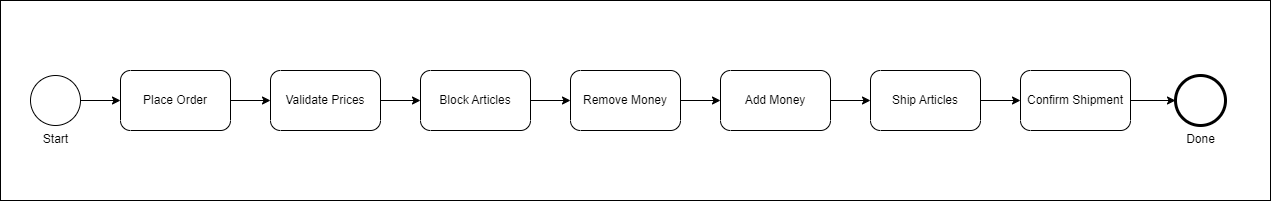
\includegraphics[width=\linewidth]{figures/SimplifiedBusinessProcess.png}
\end{figure}


% TODO Diagramm für den vereinfachten Prozess

Die zum Prozess gehörenden Schritte sind folgende:

\subparagraph*{Entgegennehmen der Bestellung} Die Bestellung wird über ein imaginäres Frontend entgegengenommen. Dieses Frontend baut einen Request auf und sendet diesen per Http-Schnittstelle an das Backend. Dort wird der Request entgegengenommen und muss alle für die Abwicklung der Bestellung erforderlichen Daten enthalten. Dazu gehören der bestellende Nutzer, die geforderten Artikel und die Zahlungsinformationen. Beim Entgegennehmen wird die Bestellung initialisiert.

\subparagraph*{Validierung des Preises} Der Bestellungsrequest enthält eine Liste von den gewünschten Produkten und dem bekannten Preis pro Produkt. Um zu überprüfen, ob der dem Nutzer (dem Frontend) bekannte Preis mit dem aktuellen Preis übereinstimmt, muss dieser validiert werden. % TODO warum ist dieser Schritt notwendig	

\subparagraph*{Blockieren der Artikel} Die geforderten Artikel sollten für diese Bestellung reserviert werden, bis der Bestellvorgang abgeschlossen ist. In einem Online-Shop wird angezeigt, wieviele Artikel auf Lager vorrätig sind. Beim Blockieren der Artikel wird dieser Betrag verändert. Somit sehen andere Nutzer nach Ausführung dieses Schrittes den aktuellen Wert der vorrätigen Artikel. 

\subparagraph*{Zahlungsabwicklung} Der berechnete Preis der Bestellung muss vom Konto des Kunden abgebucht werden. Das Konto des Händlers erhält denselben Betrag gutgeschrieben. Die Konten des Kunden und des Online-Shop-Besitzers müssen nicht bei derselben Bank liegen. 

\subparagraph*{Auslösen der Lieferung} Die blockierten Artikel werden versendet. Dieser Prozess dauert einen längeren Zeitraum an.

\subparagraph*{Abschluss der Lieferung} Der Lieferant bestätigt die Übergabe der Waren an den Kunden.


\paragraph*{Implementierung}

Nachdem der Geschäftsprozess definiert wurde, soll das Saga-System implementiert werden. In \ref{sec_saga_formalisierung_dea} wurde erläutert, wie die im Koordinator laufende SEC beschrieben werden kann. Die Implementierung soll durch diese Darstellungsform beschrieben werden können.

Für die Transaktionsteilnehmer gilt zu Beginn der Implementierung lediglich die Anforderung, dass die Schnittstellen per Request-Response-Muster aufgerufen werden. Dafür wird das Http-Protokoll verwendet.


\subsection{Schritt 2 - Messung der verschiedenen Implementierungen}

Die Bewertung der Implementierungen soll auf Grundlage von Messdaten erfolgen. Es soll nun beschrieben werden, wie die Erfassung dieser Daten erfolgen soll.

% TODO Testpyramide

\paragraph*{Systemtest} \mbox{}\\
Die Messdaten erfolgen in einer produktionsähnlichen Umgebung im Rahmen von Systemtests. Das erwartete Ergebnis ist ein konkreter Endzustand, der erreicht werden soll. Dieser Endzustand kann mit dem erreichten Endzustand verglichen werden.

\paragraph*{Testkonfiguration} \mbox{}\\
Ein solcher Systemtest wird unter einer bestimmten Konfiguration durchgeführt. Die Konfiguration setzt sich zusammen aus einem Testcase und einem Netzwerkszenario. 

\paragraph*{Testcase} \mbox{}\\
Ein Testcase stellt eine konkrete Interaktion mit dem System dar. Die Testcases übernehmen die Aufgabe, die verschiedenen Fälle der Geschäftslogik auf Korrektheit zu überprüfen.

\paragraph*{Netzwerkszenarien} \mbox{}\\
Ein Netzwerkszenario ist ebenfalls Teil der Testkonfiguration. Wird ein Systemtest durchgeführt, so beschreibt das Netzwerkszenario das konkrete Netzwerkverhalten.

% TODO wie misst man Konsistenz
\paragraph*{Messgegenstand} \mbox{}\\
Das Ziel der Messung ist, Aussagen über die Konsistenz des Systems zu treffen. In Abschnitt \ref{} wurden verschiedene Vorgehensweisen dargestellt, wie die Konsistenz eines Systems gemessen werden kann. 

Die verwendete Implementierung per Orchestrierung setzt das Vorhandensein eines Koordinators voraus. Die darin befindliche Steuerung der LLT durch die SEC gibt Auskunft über die ausgeführten lokalen Transaktionen einer Saga. Es kann für jede lokale Transaktion gemessen werden, wie oft die SEC davon ausgeht, dass eine Transaktion ausgeführt wurde. Analog dazu kann die tatsächlich ausgeführte Anzahl an Transaktionen bestimmt werden, indem die Sicht der Transaktionsteilnehmer verwendet wird. Stimmen die korrespondierenden Werte aller lokalen Transaktionen in beiden Sichten überein, kann davon ausgegangen werden, dass die LLT keine Inkonsistenzen in das System eingeführt hat.

Ein weiterer Anhaltspunkt für Konsistenzanomalien ist der erreichte Endzustand einer Transaktion. In \ref{sec_saga_formalisierung_dea} wurde ein Endzustand für einen DEA definiert, der erreicht wird, nachdem eine Saga in einer kompensierenden Aktion eine Fehlerantwort erhält. In solchen Fällen ist der Koordinator nicht in der Lage die LLT abzuschließen und endet in einem weder erfolgreichen noch kompensierten Zustand. 

Da dieser Zustand einen Fall aufzeigt, in dem die Atomarität der LLT verletzt wird, ist das Auftreten solcher Endzustände ein unmittelbares Zeichen für Inkonsistenz.

\paragraph*{Metriken} \mbox{}\\
% TODO
TODO Beschreibung, wie die Messdaten in eine (oder mehrere) Kennzahlen umgewandelt wird
\subsection{Analyse der Messdaten}
Die Ergebnisse aus der Messung stellen die Grundlage für eine Analyse des implementierten Systems dar. Die Messwerte geben Auskunft über Konsistenz, Laufzeit und Erfolgsrate. Die Werte sollen interpretiert werden. Es sind Ursachen für Konsistenzanomalien, übermäßig lange oder unbeendete Ausführungen sowie erfolglose LLTs zu identifizieren. 






%Was mache ich in dem praktischen Teil
%- was ist das ziel?
%	- zusammenhänge zwischen konsistenz und schnittstellendesign erkennen
%	- these beantworten: können Netzwerkpartitionen in Sagapattern einbezogen werden
%- methodik
%	- schritt 1: entwurf+impl eines gp
%		- anforderungen an den Gp definieren
%		- 
%	- schritt 2: durchführung von messungen 
%		- was wird gemessen?
%			- erreichte endzustände (entspricht der Sicht des Koordinators)
%			- ausgeführte Transaktionen aus Sicht des Koordinators und der Teilnehmer	
%		- unter welchen Bedingungen wird gemessen?
%			- Szenario 1, 2, 3
%			- wie werden diese Bedingungen geschaffen
%		- welche Usecases werden für die Messungen durchgeführt
%			- UC 1, 2
%	- schritt 3: 
%		- Analyse der Werte
%		- Schlüsse ziehen








